\documentclass[a4paper,12pt]{article}

\usepackage{latexsym}
\usepackage[utf8]{inputenc}
\usepackage[T1]{fontenc}
\usepackage{graphicx}
\usepackage{amsmath}
\usepackage{float}% If comment this, figure moves to Page 2
\usepackage[hidelinks]{hyperref}
\usepackage{lipsum}

\author{Krzysztof~Palka and Dominik~Odrowski}
\date{April 25, 2013}

\title{\textsc{Exercise} 346 \\ Examination of permittivity of ferroelectricity} 

\addtolength{\textwidth}{2.5cm}
\addtolength{\hoffset}{-1.25cm}

\begin{document}

    \maketitle

    \begin{abstract}
        This report presents measurement of the permittivity of ferroelectricity material using parallel-plate capacitor.
    \end{abstract}

    \section{Introduction}
    The aim of this exercise was to determine, using experimental setup mainly based on capacitor, the Curie-Weiss temperature, dependency of permittivity from temperature in paraelectric and ferroelectric phase and in general to acquaint with properties of ferroelectric materials. 

    \section{Theory and measurement}

    

    Electric permittivity can be determinate by measurement capacitance of capacitor $C$, which plates stick to plate cut form examined substance. As thickness of examined material is much less then it's area $S$ we can calculate capacitance form formula for capacitor with 2 parallel plates. Transformation of this equation lets us to calculate electric permittivity form equation:    
    \begin{equation}
        \epsilon = \frac{d C}{S \epsilon_0} \label{eq:epsilon}
    \end{equation}

    Near temperature of phase transition form ferroelectric to paraelectric permittivity can be described by Curie-Weiss low:    
    \begin{equation}
        \epsilon = \frac{K}{T-T_c} \label{eq:curie}
    \end{equation}
    where $K$ is Curie-Weiss constant. According to that inverse of permittivity is proportional to temperature  
    \begin{equation}
        \frac{1}{\epsilon} = \frac{1}{K} T - \frac{T_c}{K} \label{eq:curie2}
    \end{equation}
    It allows us to determine constans $T_c$ and $K$, lets assume following factors:  
    \begin{equation}
        \frac{1}{\epsilon} = mT + b \label{eq:curie3}
    \end{equation}
    So respectively:    
    \begin{equation}
        K = \frac{1}{m} \label{eq:k}
    \end{equation}
    and 
    \begin{equation}
        T_c = - K b \label{eq:tc}
    \end{equation}
    

    \section{Results}

    For calculation of $\epsilon$ we have used following parameters read form experimental set-up: $S = 89 \mathrm{mm}^2$, $d = 1.1$ mm. To read capacitance we have added additional capacitance form electric connections, meters etc. This value also was given and was equal approximately 48 pF.  


    \begin{table}[H]
        \begin{center}
            \caption{Measured temperature $T$, capacitance $C$ and calculated permittivity $\epsilon$ and inverse of permittivity $\epsilon^{-1}$}
            \label{tab:vn}
    
            \begin{tabular}{|c|c|c|c||c|c|c|c|}
                \hline
                $T$ [K] & $C$ [pF] & $\epsilon$ & $\epsilon^{-1}$ [$10^{-3}$] &
                $T$ [K] & $C$ [pF] & $\epsilon$ & $\epsilon^{-1}$ [$10^{-3}$] 
                \\ \hline
342.5 & 127.2 & 242.0 & 4.133 & 320.5 & 2197.0 & 3100.4 & 0.323\\
340.5 & 130.4 & 246.4 & 4.059 & 318.5 & 1573.1 & 2238.8 & 0.447\\
338.5 & 144.5 & 265.9 & 3.762 & 316.5 & 1304.6 & 1868.0 & 0.535\\
336.5 & 150.0 & 273.4 & 3.657 & 314.5 & 1136.6 & 1636.0 & 0.611\\
334.5 & 165.9 & 295.4 & 3.385 & 312.5 & 1009.4 & 1460.3 & 0.685\\
332.5 & 184.5 & 321.1 & 3.114 & 310.5 & 911.9 & 1325.7 & 0.754\\
330.5 & 217.0 & 366.0 & 2.732 & 308.5 & 833.8 & 1217.8 & 0.821\\
328.5 & 255.2 & 418.7 & 2.388 & 306.5 & 765.8 & 1123.9 & 0.890\\
326.5 & 325.5 & 515.8 & 1.939 & 304.5 & 715.6 & 1054.6 & 0.948\\
324.5 & 436.9 & 669.7 & 1.493 & 302.5 & 672.7 & 995.3 & 1.005\\
322.5 & 883.5 & 1286.4 & 0.777 & 301.1 & 636.3 & 945.0 & 1.058\\
                \hline
            \end{tabular}
        \end{center}
    \end{table}

    For linear approximation we have used points form 320.5 K to 332.5 K.

    \begin{figure}[H]
    \begin{center}
        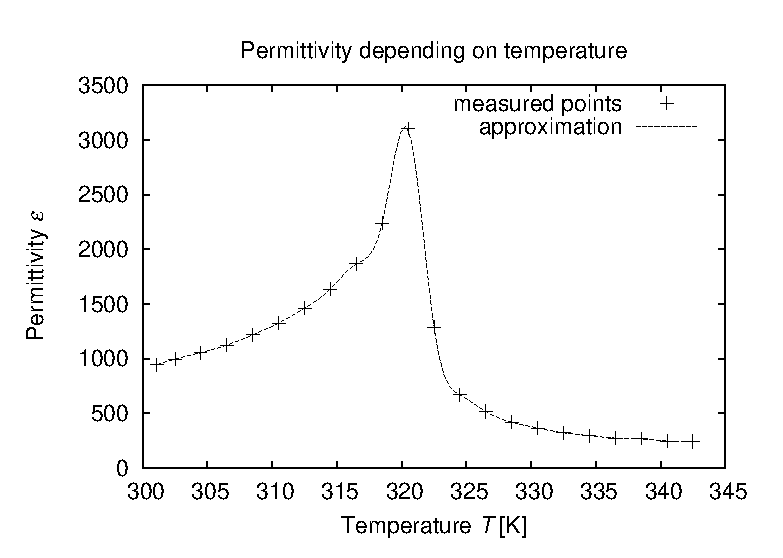
\includegraphics[width=0.7\textwidth]{epsilon}
        \caption{Graph of permittivity for measured temperature}
        \label{fig:epsilon}
    \end{center}
    \end{figure}

    \begin{figure}[H]
    \begin{center}
        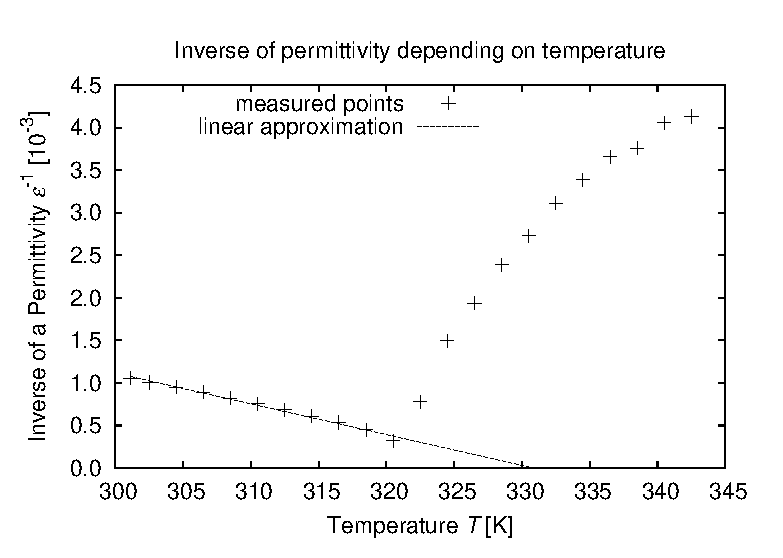
\includegraphics[width=0.7\textwidth]{epsilon-1}
        \caption{Graph of inverse of permittivity for measured temperature}
        \label{fig:epsilon-1}
    \end{center}
    \end{figure}

    Usage of least square regression for paraelectric state of of material gives
    factors $m = (2.4 \pm 0.2) \cdot 10^{-1}$ and $b = (12.0 \pm 0.4) \mathrm{K}$.
    Substituting those values to equations \ref{eq:k} and \ref{eq:tc}, we have
    obtained results:

    \begin{displaymath}
        K = \frac{1}{2.4 \cdot 10^{-4}} \approx 4.166 \cdot 10^3    
    \end{displaymath}

    and 

    \begin{displaymath}
        T_c = -1 \cdot 4.166 \cdot 10^3 \cdot 7.5 \cdot 10^{-2} \mathrm{K} \approx 312.5 \mathrm{K}
    \end{displaymath}

    Propagation of error can be calculated form equations: 

    \begin{equation}
        \Delta K = K \frac{\Delta a}{a}
    \end{equation}
    
    \begin{equation}
        \Delta T_c = T_c \left( \frac{\Delta K}{K} + \frac{\Delta b}{|b|} \right)
    \end{equation}
    
    So complete results are as following

    \begin{displaymath}
        K = (4.2 \pm 0.4) \cdot 10^3
    \end{displaymath}
    
    \begin{displaymath}
        T_c = (3.1 \pm 0.5) \cdot 10 ^ 2 K
    \end{displaymath}
    


    \section{Conclusions}

    As we can observe on graph \ref{fig:epsilon-1} even though we have chose
    those points, which seemed to be quite linear, obtained uncertainty is 
    huge. We have found 2 possible materials with such Curie temperature: 
    Gd (gadolinium, 293K) and MnAs (combination of arsen and mangan, 318K)
    \cite{res}. There was couple factors that inflated on results, for example
    precision of termometr, location of it sensor, additional capacitance of
    set-up. Using formula for capacitor with 2 parallel plates could affect
    result, but not in significant way. Other reason could be not sufficient
    resolution of measurement, 2 K in this case could led to bigger errors.  

    \begin{thebibliography}{9}


        \bibitem{res}\emph{Handbuch der Physik} (1966) F. Keffer. New York: Springer-Verlag. Cite available online at: \url{http://hyperphysics.phy-astr.gsu.edu/hbase/tables/curie.html}. Accessed April 29, 2013.

    \end{thebibliography}

\end{document}
